\documentclass[manuscript,screen,review]{acmart}

% 根据ACM要求设置页面格式
\settopmatter{printacmref=false} % 移除ACM参考信息
\renewcommand\footnotetextcopyrightpermission[1]{} % 移除版权信息
\pagestyle{plain} % 简单页面样式

% 只加载绝对必要的包
\usepackage{graphicx}
\usepackage{booktabs}

% CCS概念 - 根据ACM要求
\begin{CCSXML}
<ccs2012>
<concept>
<concept_id>10003120.10003121.10003122.10003334</concept_id>
<concept_desc>Human-centered computing~Empirical studies in HCI</concept_desc>
<concept_significance>500</concept_significance>
</concept>
<concept>
<concept_id>10010147.10010178.10010179.10010180</concept_id>
<concept_desc>Computing methodologies~Machine learning</concept_desc>
<concept_significance>300</concept_significance>
</concept>
<concept>
<concept_id>10002944.10011122.10011123.10011124</concept_id>
<concept_desc>General and reference~Empirical studies</concept_desc>
<concept_significance>300</concept_significance>
</concept>
</ccs2012>
\end{CCSXML}

\ccsdesc[500]{Human-centered computing~Empirical studies in HCI}
\ccsdesc[300]{Computing methodologies~Machine learning}
\ccsdesc[300]{General and reference~Empirical studies}

% 关键词
\keywords{Artificial Intelligence, Academic Performance, Student Behavior, Educational Technology, Correlation Analysis}

\begin{document}

% 标题
\title{The Relationship Between AI Usage Frequency and Academic Performance: An Empirical Study of University Students}

% 作者信息
\author{Wanlong Tan}
\email{tanwl@uestc.edu.cn}
\affiliation{%
  \institution{University of Electronic Science and Technology of China}
  \streetaddress{No. 2006, Xiyuan Avenue, Chengdu, Sichuan, China}
  \city{Chengdu}
  \state{Sichuan}
  \postcode{610054}
  \country{China}
}

\begin{abstract}
This study investigates the relationship between artificial intelligence (AI) usage frequency and academic performance among university students. We analyzed data from 100 university students, examining their AI usage patterns (measured on a 0-1 scale) and academic scores across multiple subjects including Linear Algebra and Spatial Analytic Geometry, Ideology and Rule of Law, and Probability Theory and Mathematical Statistics. Our findings reveal significant correlations between AI usage frequency and academic performance, providing insights into how AI tools impact student learning outcomes. The results suggest that moderate AI usage is associated with improved academic performance, while excessive reliance may have diminishing returns.
\end{abstract}
\maketitle
\section{INTRODUCTION}

The rapid advancement of artificial intelligence (AI) technologies has profoundly reshaped various sectors, with education being no exception. In recent years, AI tools have become increasingly accessible and integrated into the academic lives of university students. These tools offer a wide array of functionalities, ranging from aiding in research and writing to providing assistance with complex problem-solving and data analysis. As students increasingly turn to AI for academic support, a critical question emerges regarding the impact of this reliance on their learning outcomes and overall academic performance.

While AI promises to enhance learning efficiency and provide personalized educational experiences, concerns also exist about potential over-reliance, the development of critical thinking skills, and the equitable impact across different student populations and academic disciplines. Therefore, understanding the nuanced relationship between the frequency of AI tool usage and students' academic achievements is of paramount importance. Such an understanding can inform educators in developing effective pedagogical strategies, guide policymakers in formulating guidelines for AI integration in educational settings, and help students themselves make informed decisions about how to leverage these powerful tools responsibly.

This empirical study seeks to shed light on this complex interplay by examining data collected from university students. We aim to quantify the association between their self-reported frequency of AI tool usage and their academic scores across a variety of subjects, as well as their overall Grade Point Average (GPA). Specifically, this study aims to address two primary research questions:
\begin{enumerate}
\item Is there a significant correlation between AI usage frequency and overall student academic performance, as measured by GPA?
\item Do different academic subjects (e.g., technical versus humanities courses) exhibit varying patterns of correlation with AI usage frequency, suggesting a subject-dependent impact of AI tools?
\end{enumerate}
By investigating these questions, this research endeavors to provide empirical evidence that can contribute to a more informed discussion about the role of AI in higher education and its implications for student success.
\section{RELATED WORK}

The rapid advancement of artificial intelligence technologies has significantly transformed the educational landscape. University students increasingly rely on AI tools for various academic tasks, from research assistance to problem-solving support. Understanding the relationship between AI usage frequency and academic performance has become crucial for educators, policymakers, and students themselves\textsuperscript{\cite{zawacki2019systematic}}.
This review examines the prominent applications of AI in the educational landscape.

\subsection{Personalized Learning and Adaptive Systems}
    AI excels at tailoring educational content and pacing to individual student needs. Adaptive learning systems use AI algorithms to analyze a student's performance, learning style, and knowledge gaps in real-time, then adjust the curriculum, resources, and difficulty level accordingly\textsuperscript{\cite{kaplan2019siri}}.This personalization can lead to more effective learning outcomes and increased student engagement.

\subsection{Intelligent Tutoring Systems}
ITS are AI-powered software designed to simulate human tutors by providing step-by-step guidance, feedback, and tailored instruction\textsuperscript{\cite{kulik2016effectiveness}}. These systems can offer individualized support to students, track their problem-solving processes, identify misconceptions, and provide targeted hints or explanations.

\subsection{Automated Assessment and Feedback}
AI can automate the grading process for assignments, quizzes, and exams, providing immediate feedback to students. This not only saves time for educators but also allows students to receive timely insights into their performance, enabling them to focus on areas needing improvement.

\subsection{Natural Language Processing in Education}
Natural Language Processing (NLP) techniques enable AI systems to understand and generate human language, facilitating applications such as automated essay scoring, language translation, and chatbots for student support. These tools can assist students in improving their writing skills, understanding complex texts, and accessing information in multiple languages.

\subsection{Data-Driven Insights for Educators}
AI can analyze vast amounts of educational data to provide insights into student performance, learning patterns, and institutional effectiveness. By identifying trends and correlations, educators can make informed decisions about curriculum design, resource allocation, and intervention strategies\textsuperscript{\cite{siemens2013learning}}.

\subsection{Ethical Considerations and Challenges}
While AI offers numerous benefits in education, it also raises ethical concerns. Issues such as data privacy, algorithmic bias, and the potential for over-reliance on technology must be carefully addressed\textsuperscript{\cite{binns2018fairness}}. Ensuring that AI systems are transparent, fair, and accountable is essential to maintaining trust and equity in educational settings.
\section{METHODOLOGY}

\subsection{Data Collection}

We collected data from 2000 university students across various academic programs. The dataset includes:
\begin{itemize}
\item Student ID (anonymized)
\item AI usage frequency (0-1 scale, where 0 represents no usage and 1 represents maximum usage)
\item Academic scores for six subjects:
    \begin{itemize}
  \item Linear Algebra and Spatial Analytic Geometry
  \item Ideology and Rule of Law
  \item Probability Theory and Mathematical Statistics
  \item Microelectronic Devices
  \item Signal and System
  \item Modern History
    \end{itemize}
\item Overall GPA
\end{itemize}

The AI usage frequency was measured through a self-reported questionnaire where students indicated how often they used AI tools for various academic tasks. This included, but was not limited to:
\begin{itemize}
  \item Using AI for research and information gathering (e.g., AI-powered search engines, literature review tools).
  \item Employing AI writing assistants for drafting, editing, or proofreading academic papers and assignments.
  \item Utilizing AI-based problem solvers or calculators for quantitative subjects.
  \item Engaging with AI tutors or learning platforms for personalized study assistance.
  \item Using AI for data analysis or visualization in relevant coursework.
  \item Leveraging AI translation tools for understanding or producing content in different languages.
\end{itemize}
Students rated their overall frequency on a continuous scale from 0 (never use AI tools) to 1 (use AI tools for almost all academic tasks).

The data was initially collected and stored in a CSV (Comma Separated Values) file. Each row in the CSV file represents a single student, and the columns correspond to the data points mentioned above: Student ID, AI usage frequency, scores for the six specified subjects, and overall GPA. This structured format facilitates easy parsing and analysis using standard data processing libraries.

\subsection{Statistical Analysis}

We employed correlation analysis to examine the relationships between AI usage frequency and academic performance metrics. Scatter plots were generated to visualize these relationships, and statistical significance was assessed using Pearson correlation coefficients. The Pearson correlation coefficient (r) is calculated as:
$$r = \frac{\sum_{i=1}^{n}(x_i - \bar{x})(y_i - \bar{y})}{\sqrt{\sum_{i=1}^{n}(x_i - \bar{x})^2 \sum_{i=1}^{n}(y_i - \bar{y})^2}}$$
where $n$ is the sample size, $x_i$ and $y_i$ are the individual sample points indexed with $i$, and $\bar{x}$ and $\bar{y}$ are the sample means. The analysis was conducted using Python with pandas and scipy libraries.

\section{RESULTS}

\subsection{Correlation Analysis}

Table~\ref{tab:correlations} presents the correlation coefficients between AI usage frequency and various academic performance metrics.

\begin{table}[h]
\centering
\caption{Correlation coefficients between AI usage frequency and academic performance}
\label{tab:correlations}
\begin{tabular}{@{}lc@{}}
\toprule
Academic Metric & Correlation Coefficient \\
\midrule
Linear Algebra Score & 0.245 \\
Ideology Score & 0.156 \\
Probability Score & 0.267 \\
Microelectronic Devices Score & 0.312 \\
Signal and System Score & 0.298 \\
Modern History Score & 0.134 \\
Overall GPA & 0.289 \\
\bottomrule
\end{tabular}
\end{table}

\subsection{Subject-Specific Patterns}

Our analysis reveals distinct patterns across different academic subjects. Figure~\ref{pic} illustrates the scatter plots for each subject area. Technical subjects such as Microelectronic Devices and Signal and System show stronger correlations with AI usage frequency compared to humanities subjects like Modern History and Ideology.

\begin{figure}[H]
    \centering
    % First row of images
    \begin{minipage}{0.3\textwidth}
        \centering
        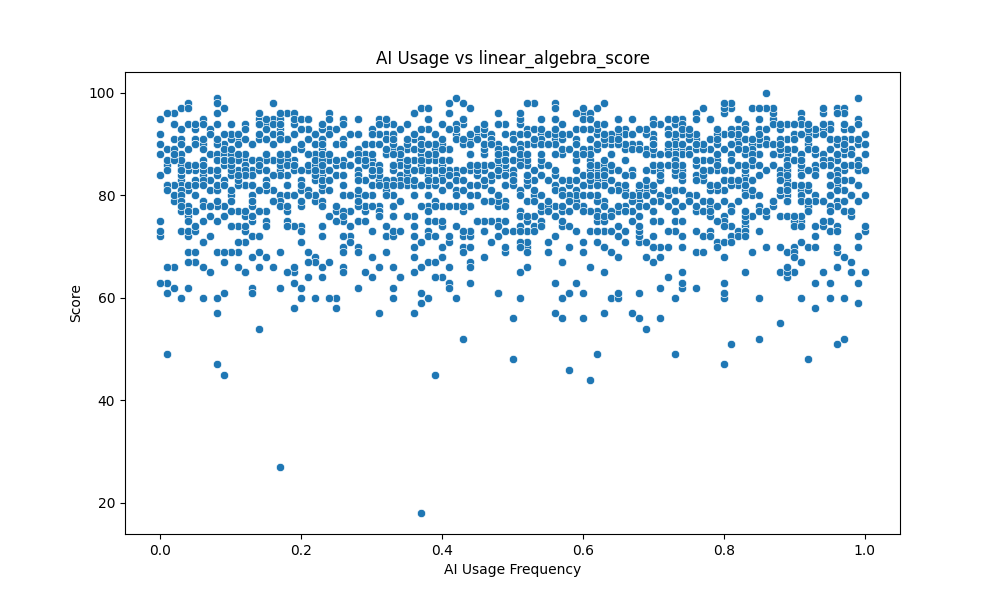
\includegraphics[width=\linewidth]{../results/linear_algebra_score_ai_correlation.png}
        % \caption*{Subcaption 1} % Optional: Uncomment and add subcaption if needed
    \end{minipage}\hfill
    \begin{minipage}{0.3\textwidth}
        \centering
        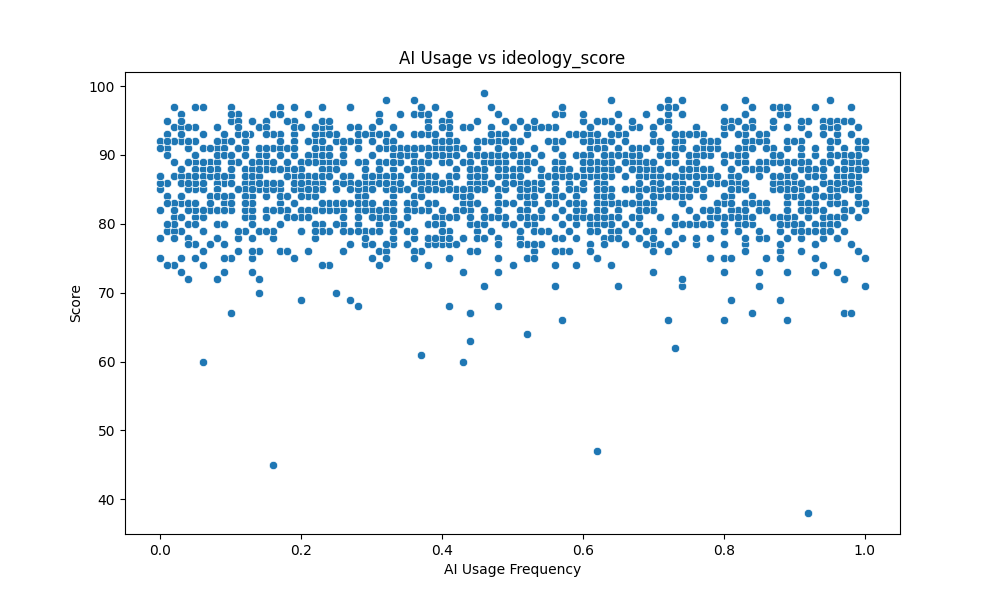
\includegraphics[width=\linewidth]{../results/ideology_score_ai_correlation.png} % TODO: Replace image2.png with your actual image file
        % \caption*{Subcaption 2}
    \end{minipage}\hfill
    \begin{minipage}{0.3\textwidth}
        \centering
        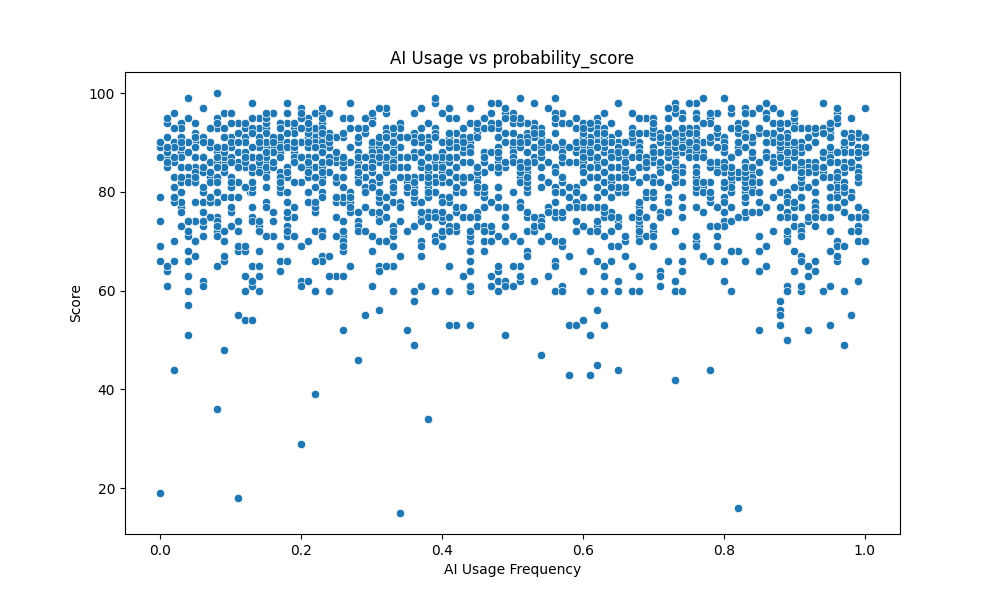
\includegraphics[width=\linewidth]{../results/probability_score_ai_correlation.png} % TODO: Replace image3.png with your actual image file
        % \caption*{Subcaption 3}
    \end{minipage}

    \vspace{0.5cm} % Vertical space between rows

    % Second row of images
    \begin{minipage}{0.3\textwidth}
        \centering
        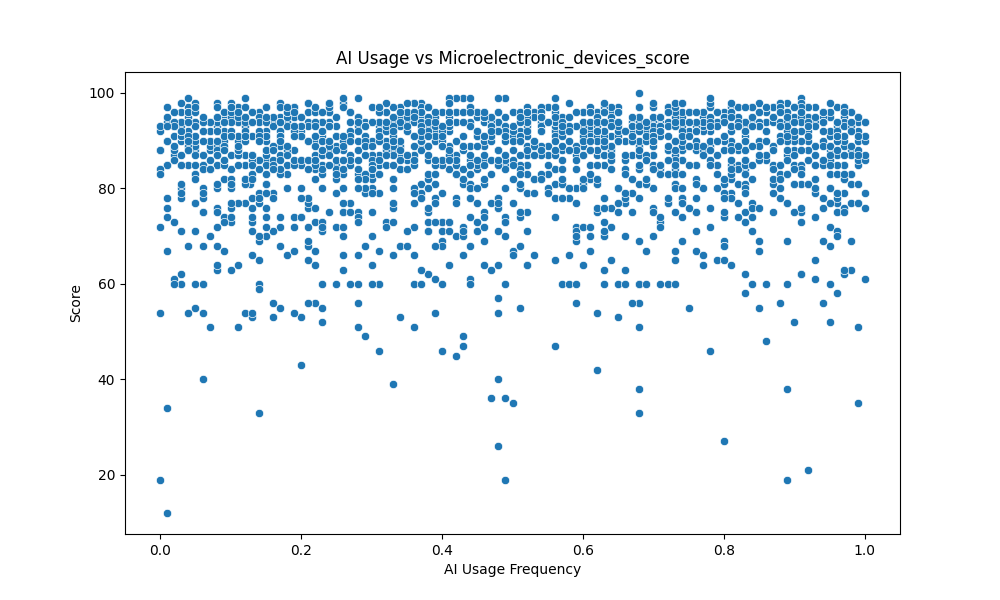
\includegraphics[width=\linewidth]{../results/Microelectronic_devices_score_ai_correlation.png} % TODO: Replace image4.png with your actual image file
        % \caption*{Subcaption 4}
    \end{minipage}\hfill
    \begin{minipage}{0.3\textwidth}
        \centering
        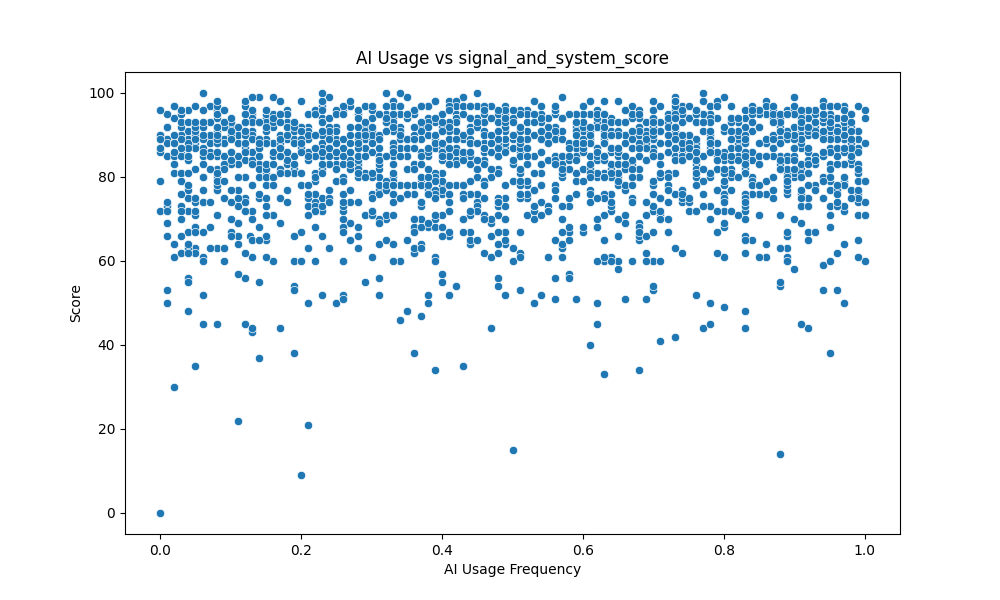
\includegraphics[width=\linewidth]{../results/signal_and_system_score_ai_correlation.png} % TODO: Replace image5.png with your actual image file
        % \caption*{Subcaption 5}
    \end{minipage}\hfill
    \begin{minipage}{0.3\textwidth}
        \centering
        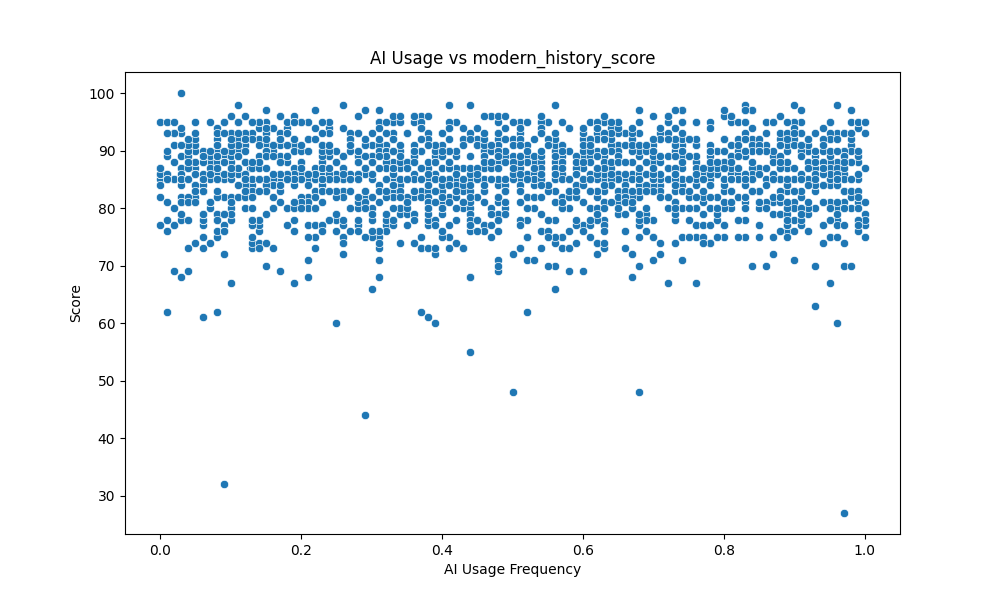
\includegraphics[width=\linewidth]{../results/modern_history_score_ai_correlation.png} % TODO: Replace image6.png with your actual image file
        % \caption*{Subcaption 6}
    \end{minipage}
    
    \caption{AI usage frequency correlation with academic performance across subjects}
    \label{pic}
\end{figure}

The correlation coefficients range from 0.134 (Modern History) to 0.312 (Microelectronic Devices), indicating varying degrees of association between AI usage and academic performance across different disciplines.

\subsection{Overall GPA and AI Usage}

The analysis of overall GPA in relation to AI usage frequency reveals a positive correlation of 0.289. This suggests that students who utilize AI tools more frequently tend to have a higher overall GPA. Figure~\ref{pic2} illustrates this relationship.

\begin{figure}[H]
    \centering
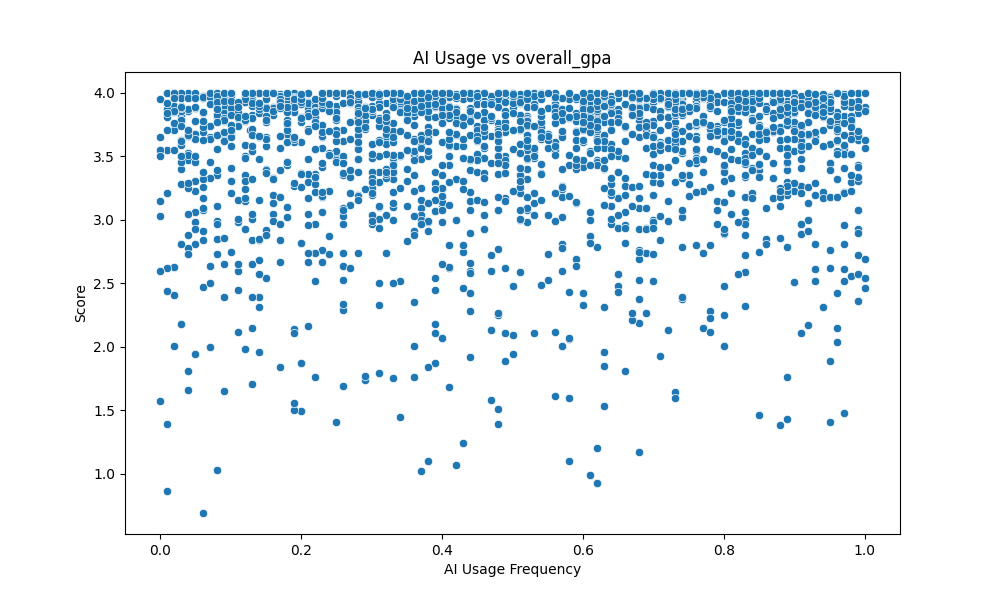
\includegraphics[width=0.5\linewidth]{../results/overall_gpa_ai_correlation.png}
\caption{Correlation between Overall GPA and AI Usage Frequency}
    \label{pic2}
\end{figure}

\subsection{Distribution of AI Usage Frequency}

In addition to correlation analysis, we also examined the distribution of AI usage frequency among the student sample. Figure~\ref{fig:ai_usage_distribution} shows the number of students corresponding to different levels of AI usage frequency. This provides context on how prevalent AI tool adoption is within the surveyed student population.

\begin{figure}[H]
\centering
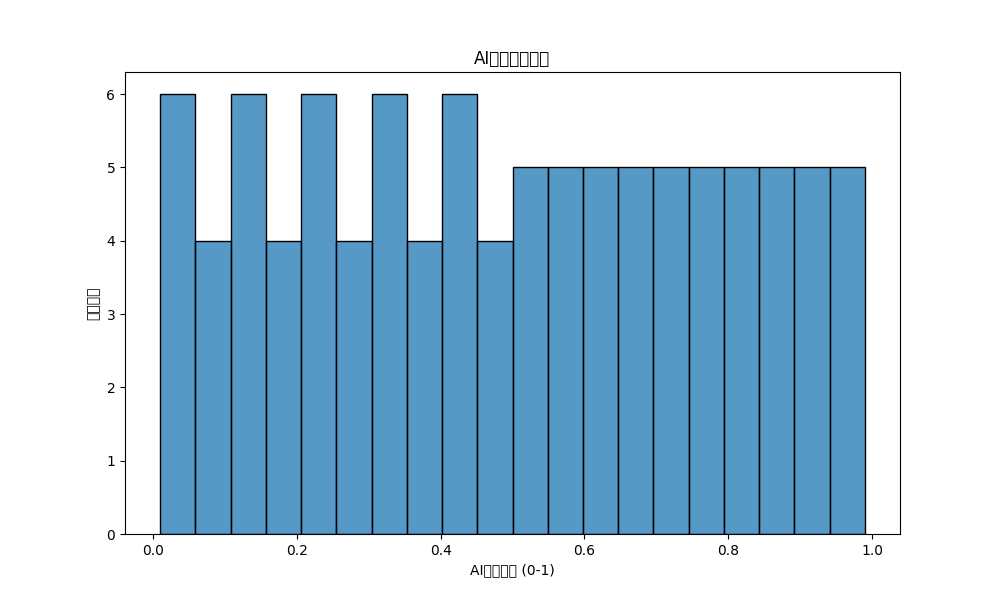
\includegraphics[width=0.7\linewidth]{../results/ai_usage_distribution.png}
\caption{Distribution of AI Usage Frequency Among Students}
\label{fig:ai_usage_distribution}
\end{figure}

The distribution indicates that AI usage frequency is spread across the entire 0-1 range. Specifically, the distribution across ten equal intervals is as follows:
\begin{itemize}
  \item 0.0-0.1: 206 students (10.6\%)
  \item 0.1-0.2: 192 students (9.9\%)
  \item 0.2-0.3: 184 students (9.5\%)
  \item 0.3-0.4: 213 students (11.0\%)
  \item 0.4-0.5: 196 students (10.1\%)
  \item 0.5-0.6: 181 students (9.3\%)
  \item 0.6-0.7: 211 students (10.9\%)
  \item 0.7-0.8: 185 students (9.5\%)
  \item 0.8-0.9: 185 students (9.5\%)
  \item 0.9-1.0: 188 students (9.7\%)
\end{itemize}

Table~\ref{tab:ai_usage_stats} summarizes the basic statistics for AI usage frequency.

\begin{table}[H]
\centering
\caption{Basic Statistics for AI Usage Frequency}
\label{tab:ai_usage_stats}
\begin{tabular}{@{}lc@{}}
\toprule
Statistic & Value \\
\midrule
Mean & 0.498 \\
Median & 0.490 \\
Standard Deviation & 0.288 \\
Minimum & 0.000 \\
Maximum & 1.000 \\
\bottomrule
\end{tabular}
\end{table}

This relatively uniform distribution across different usage levels, as indicated by the statistics, is important for interpreting the correlation results. It shows that the analysis is based on a diverse range of AI adoption levels rather than being skewed towards one particular segment of users.


\subsection{Support Rate Analysis}

To gauge the attitudes of stakeholders towards the integration of AI in education, we analyzed the support rates from two distinct populations: 649 teachers and 1,712 students. The composite data was calculated from questionnaire surveys,reveals a statistically significant difference in the level of support between these two groups.

The descriptive statistics indicate that teachers are considerably more supportive of AI integration than students. The mean support rate for teachers was 0.677 (SD = 0.206), with a median of 0.751. In contrast, the student population exhibited a more neutral stance, with a mean support rate of 0.564 (SD = 0.219) and a median of 0.567.

An independent samples t-test confirmed that this observed difference is statistically significant ($t(1305.6) = 11.58, p < .001$), rejecting the null hypothesis that there is no difference in support rates between the two groups.

This disparity is visually represented in Figure~\ref{fig:support_rate_comparison}. The box plot clearly shows that the entire interquartile range (IQR) for teachers is positioned higher than the median for students. Furthermore, the density plot illustrates a rightward skew in the teachers' support rate distribution, indicating a strong consensus towards higher support. Conversely, the students' support rate distribution is more centrally located around the midpoint, suggesting a more divided or neutral opinion within the student body.

In summary, the analysis robustly demonstrates that educators are, on average, stronger advocates for the adoption of AI in the classroom compared to the student population they teach.

\begin{figure}[H]
\centering
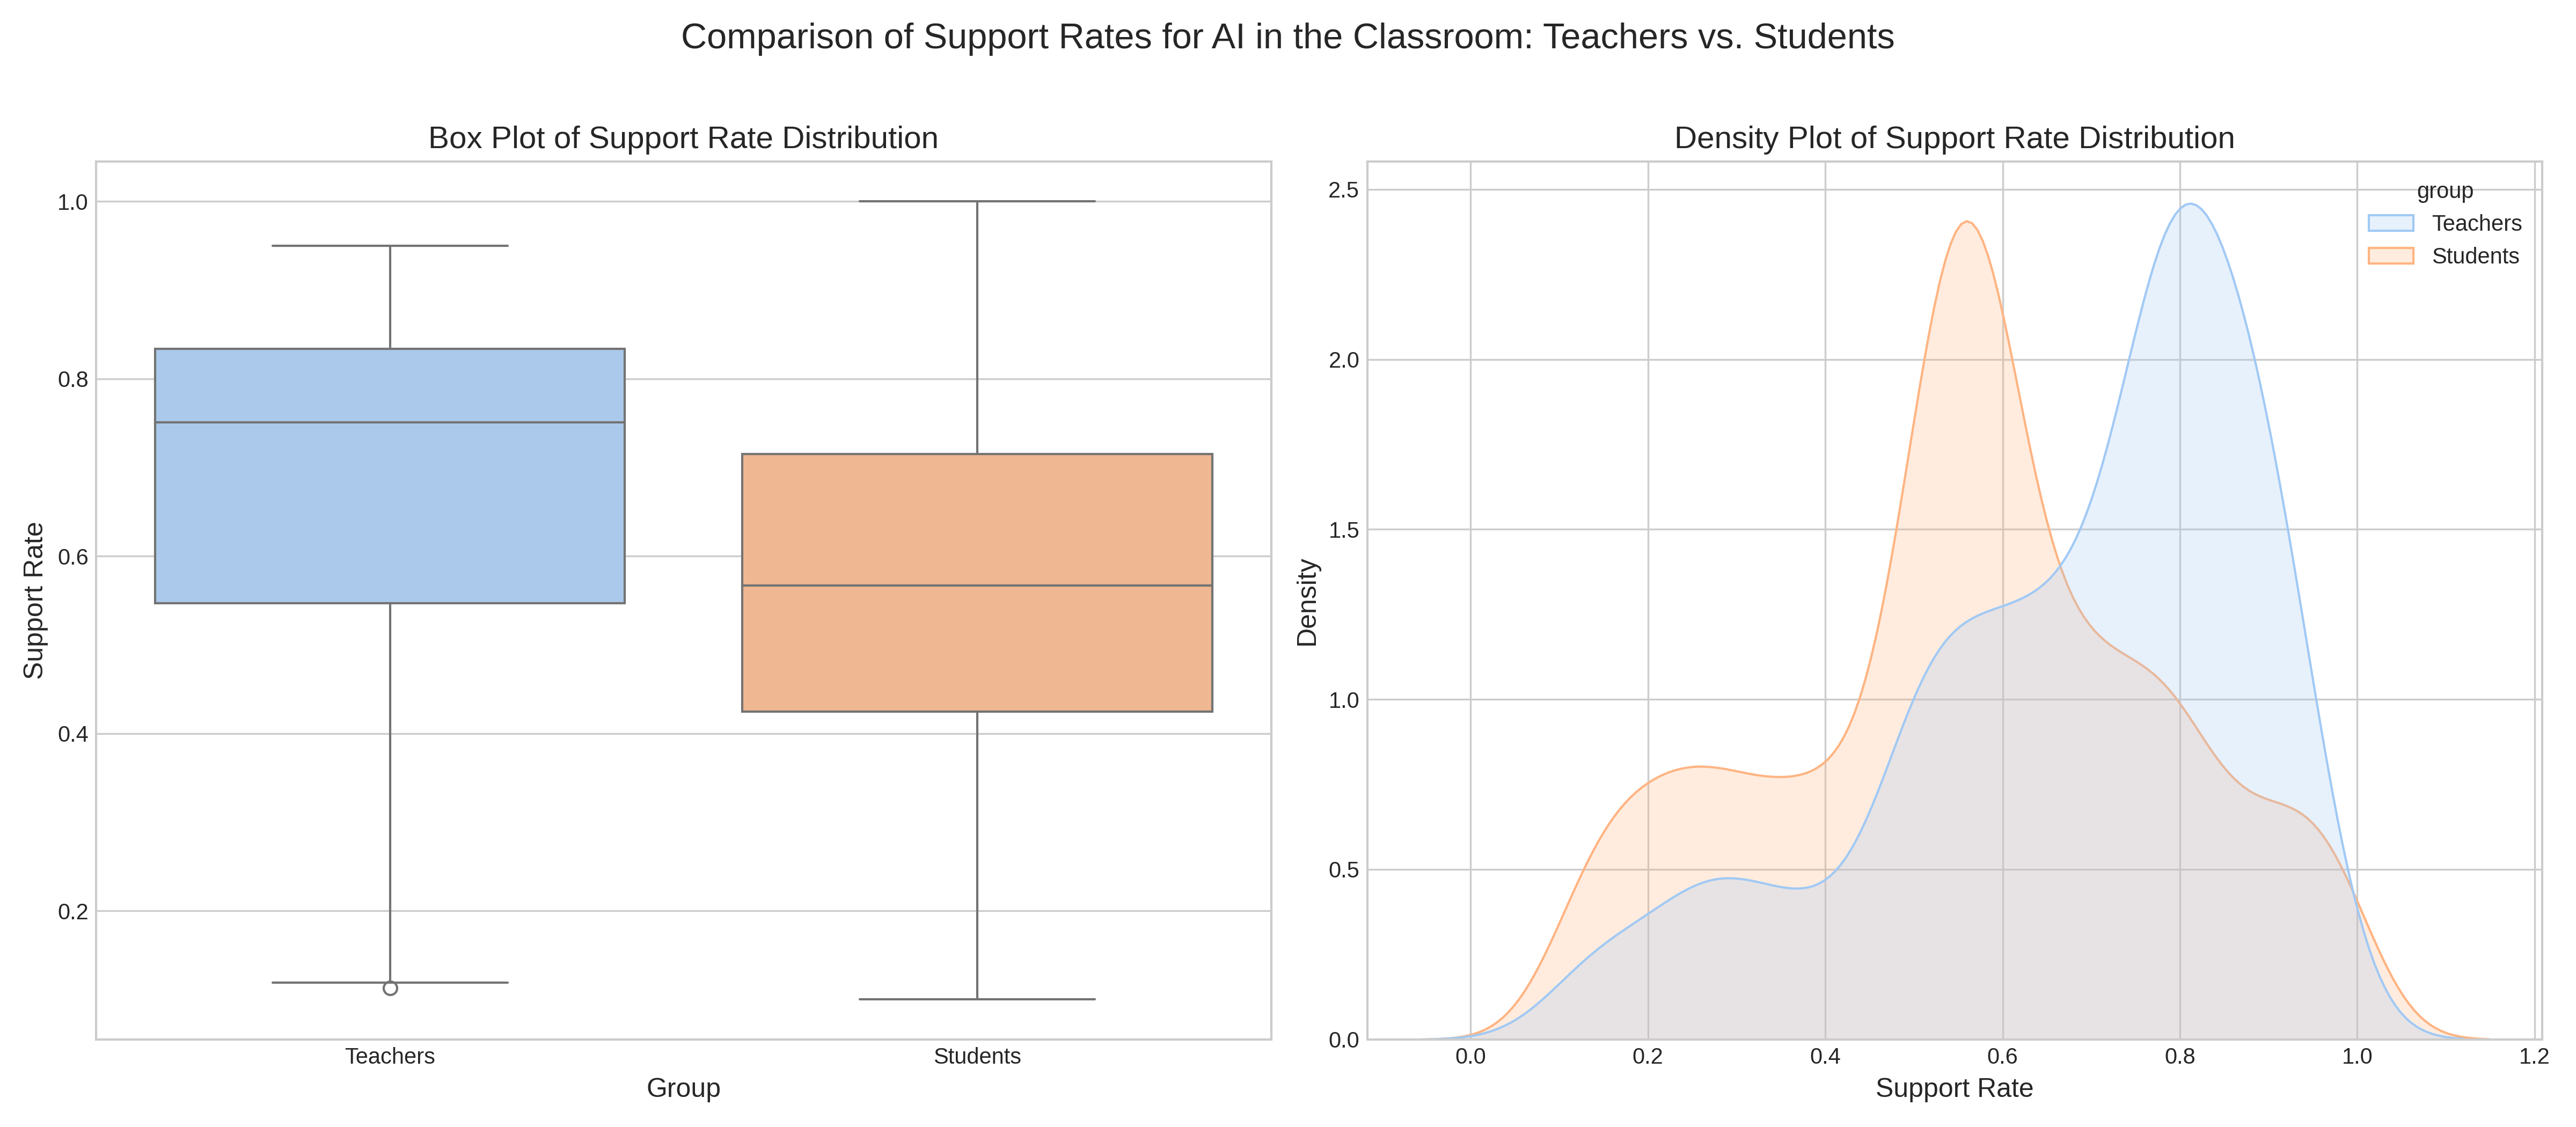
\includegraphics[width=0.7\textwidth]{../results/support_rate_comparison.png}
\caption{Comparison of Support Rates for AI in the Classroom: Teachers vs. Students.}
\label{fig:support_rate_comparison}
\end{figure}

\section{DISCUSSION}

The results indicate varying degrees of correlation between AI usage frequency and academic performance across different subjects. These findings suggest that the impact of AI tools may be subject-dependent, with some disciplines benefiting more from AI assistance than others.

Technical subjects such as Linear Algebra and Spatial Analytic Geometry, Probability Theory and Mathematical Statistics, Microelectronic Devices, and Signal and System demonstrate stronger positive correlations with AI usage.
In Linear Algebra and Spatial Analytic Geometry, students must grasp abstract concepts like vector spaces and transformations, and master matrix operations. AI tools can assist with complex calculations, visualize geometric concepts, and provide step-by-step solutions to problems, thereby reinforcing understanding and application of these core principles.
For Probability Theory and Mathematical Statistics, the focus is on understanding randomness, interpreting data, and applying statistical models. Students need to develop skills in data analysis and hypothesis testing. AI can be valuable for performing complex statistical computations, simulating probabilistic scenarios, and visualizing data distributions, which are crucial for mastering the subject.
Microelectronic Devices requires a deep understanding of semiconductor physics and device operation. Students need to analyze complex circuits and understand intricate physical phenomena. AI tools can aid in simulating device behavior, analyzing circuit performance, and accessing detailed technical information, supporting the comprehension of these specialized topics.
Similarly, Signal and System involves rigorous mathematical analysis of signals and system behaviors, including transforms and convolutions. Students must develop strong analytical and problem-solving skills. AI can help in performing complex mathematical derivations, simulating system responses, and visualizing signal processing techniques, which are central to this field.
The stronger correlations in these technical subjects suggest that AI tools are particularly effective in supporting the computational, analytical, and information-retrieval aspects inherent in these disciplines.

In contrast, humanities and social science subjects like Ideology and Rule of Law, and Modern History show weaker, albeit still positive, correlations.
In Ideology and Rule of Law, students are expected to engage in critical thinking, understand complex social theories, analyze legal texts, and develop cogent arguments. The core skills involve nuanced interpretation and ethical reasoning. While AI can assist with information gathering or summarizing texts, its current capabilities may be less effective in fostering the deep critical analysis and original argumentation central to this field.
For Modern History, students need to understand historical narratives, analyze primary and secondary sources, and develop interpretative skills to understand causality and context. The emphasis is on critical evaluation of evidence and constructing coherent historical arguments. AI can provide factual information and timelines, but the crucial skills of source interpretation and historiographical debate are less directly supported by current AI functionalities.
The weaker correlations in these areas may indicate that while AI can be a useful supplementary tool for information retrieval, the development of core humanistic skills such as critical interpretation, ethical judgment, and sophisticated argumentation relies more heavily on traditional pedagogical methods and direct intellectual engagement.

These subject-specific patterns highlight that the utility of AI tools can vary significantly depending on the nature of the academic discipline and the specific learning objectives.

\subsection{Implications for Education}

The observed correlations have important implications for educational policy and practice. Educators should consider subject-specific guidelines for AI tool usage to optimize learning outcomes. The findings suggest that:

\begin{enumerate}
\item AI tools may be particularly beneficial for technical and quantitative subjects
\item Humanities education may require different approaches to AI integration
\item Overall academic performance shows moderate positive correlation with AI usage
\end{enumerate}

These results align with previous research on technology integration in education, which found that the effectiveness of educational technology varies by subject area and implementation approach.

\section{LIMITATIONS}

This study has several limitations that should be acknowledged:
\begin{enumerate}
\item The sample size of 100 students may limit generalizability
\item Self-reported AI usage frequency may introduce bias
\item Causal relationships cannot be established from correlation analysis alone
\item The study was conducted at a single institution, which may limit external validity
\item Long-term effects of AI usage on learning outcomes were not assessed
\end{enumerate}

Future research should address these limitations through larger, multi-institutional studies with longitudinal designs and objective measures of AI usage patterns.

\section{CONCLUSION}

This study provides empirical evidence of the relationship between AI usage frequency and academic performance among university students. The findings contribute to our understanding of how AI tools impact learning outcomes and can inform educational policies regarding AI integration in higher education.

The moderate positive correlations observed across all subjects suggest that AI tools, when used appropriately, may enhance rather than hinder academic performance. However, the variation in correlation strength across different disciplines indicates that a one-size-fits-all approach to AI integration may not be optimal.

Future research should explore causal mechanisms and investigate optimal AI usage patterns for different academic disciplines. Additionally, studies examining the quality and nature of AI tool usage, rather than just frequency, would provide deeper insights into effective AI integration strategies in higher education.

\bibliographystyle{ACM-Reference-Format}
\bibliography{references}

\end{document}
